\chapter{Implementation}
\label{cha:implementation}
\epigraph{
  This chapter provides an overview over the problem we are trying to solve
  and shows how it was translated into a Tensorflow model.
  It highlights the most important technical considerations
  that were made during the implementation of the anomaly detection,
  which was described theoretically in the previous chapters. The different
  parts of the model, from input pipeline, over the ESN architecture to the
  hyper-parameter and weight optimizations, are illustrated with some brief
  pseudocode snippets.
}


\section{Development}%
\label{sec:development}

The code for this thesis was written in Numpy, Scipy, and Tensorflow.
Tensorflow [\cite{tensorflow2016}] is the most commonly used framework for
implementing ML models. It is an open source library that is maintained mostly
by Google engineers. In addition to implementing the most common GD algorithms,
from plain GD to more advanced algorithms such as Adam, Tensorflow takes care
of parallelizing and distributing the large matrix operations that make ML so
powerful.  The core design principle of Tensorflow is to separate the build and
execution phases of the model. First, the desired model architecture is
constructed by defining the \emph{computational graph}. This graph is then
optimized and during model execution certain nodes in the graph can be
requested for evaluation.  Tensorflow will then only execute the parts of the
model that are necessary to evaluate the requested node. Some of the more
intricate solutions that are presented (especially in
Sec.~\ref{sec:encoder_decoder}) might be obsolete by the time of reading, as
Tensorflow was under heavy development. It had not reached a stable API during
the main development phase of the code, which was written mainly in Tensorflow
versions 1.6-1.9.


\subsection{The Journey}%
\label{sub:the_journey}

At the beginning of this thesis it was not yet clear that the final approach
would involve reservoir computing, which does not need to make use of the very
convenient gradient and automated differentiation methods that Tensorflow
offers. However, the automatic parallelization of the network still comes in
handy. Additionally, Tensorflow comes with a tool called TensorBoard, which
makes it easy to visualize the network architecture
(Fig.~\ref{fig:network_graph}) and the learning performance during development.
A reevaluation of the advantages and drawbacks of Tensorflow and a second ML
framework called \emph{PyTorch}, that is currently gaining popularity, would
most probably lead to the choice of PyTorch over Tensorflow.  The dynamic
features that are needed to implement RNNs are accesible in a much more
pythonic way in PyTorch. Additionally, PyTorch seems to be faster at RNN tasks
than Tensorflow, but this claim was not veryfied personally. That being said,
PyTorch is still in an even earlier stage of development than Tensorflow, and
was not as popular in the beginning of this work.\\

The implementation of the algorithm that was described theoretically in the
previous chapters is the result of a search for a suitable architecture and
training method that has required numerous trial and error attempts.  The
result is a carefully orchestrated model that allows the prediction of
high-dimensional, spatio-temporal, chaotic systems. Although it should be quite
straight forward to implement a functioning ESN, with the theoretical
background that was laid in the three previous chapters, the model is quite
easy to break.  Slightly defective training procedures can lead to the
reproduction of the current time frame instead of a prediction of the future.
Once the network is correctly implemented, it still is not trivial to make it
produce sensible predictions for different datasets due to the large number of
hyper-parameters that have to be set.  Erroneous hyper-parameter setups easily
result in predictions that quickly diverge, or do nothing but decay to the mean
value of the input sequence.  Especially the last error is very hard to fix
without a good intuition of the internal dynamics of the ESN.  Tensorflow's
rather opaque RNN programming model does its part in slowing down the
resolution of these problems.



\section{The \texttt{torsk} Module}%
\label{sec:overview}

The code that was developed in this work can be found on GitHub
[\cite{coderepo}], code snippets that are presented here are partially simplified
to pseudocode to highlight only the important parts of the implementation and
reduce the amount of cited boilerplate code. The parts where this is done are
recognizable through inline comments.

The package that implements the anomaly detection is subdivided into three main
parts: \ttt{torsk.datasets} (containing functions that create input pipelines
for the different datasets), \ttt{torsk.esn} (where the ESN implementation
itself is located), and \ttt{torsk.models} (containing different network
architectures). In addition, there are two small visualization and analysis
submodules to inspect the output of the Tensorflow models.

\begin{figure}
  \centering
  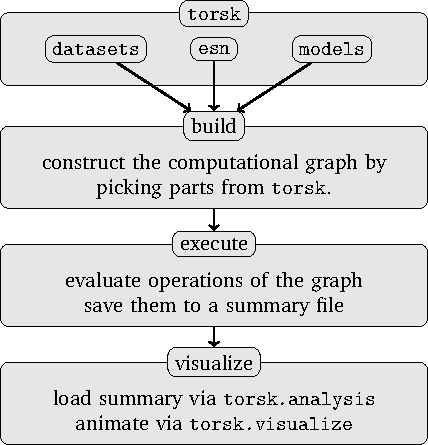
\includegraphics[width=0.5\linewidth]{tikz/flow.pdf}
  \caption{Flow chart of the algorithm}
  \label{fig:flowchart}
\end{figure}

Fig.~\ref{fig:flowchart} shows a flow chart of the whole detection algorithm,
to provide an overview over how it works.  To realize the anomaly detection in
Tensorflow, it is broken down into three phases: First, the build phase, where
the computational graph is constructed. Second, the execution phase, which
evaluates the graph in an appropriate order to optimize the ESN and make
predictions. And third, the visualization of the results.  If an online
learning model (powered by GD algorithms) is ran, then the execution and
visualization phases can also be unified.

Once the graph is constructed it is, thanks to Tensorflow, almost trivial to
pick out the operations that are desired and evaluate them. As the execution
and visualization phases of the algorithm are rather straight forward and can
be examined more closely in the examples of the \ttt{torsk} repo, the rest of
this section will focus on the build phase of the network. 


\section{Building the Computational Graph}%
\label{sec:building_the_computational_graph}

Before getting into the concrete implementation details of the graph, let us
restate what we are trying to achieve:  Based on an input sequence $\mathbf{u}$
we want to create a prediction $\mathbf{y}$ and compare this prediction to the
truth $\mathbf{d}$ so that we can identify an anomaly based on the deviation of
$\mathbf{y}$ and $\mathbf{d}$. 

This problem can be broken down in a few steps to gradually build up the
complete computational graph (Fig.~\ref{fig:network_graph}), which are listed
below.  Reminder: A frame of the input sequence $\mathbf{u}$ at time $t$ is
denoted by $\vt{u}$ (analogous for $\mathbf{y}$ and $\mathbf{d}$).

\begin{figure}
  \centering
  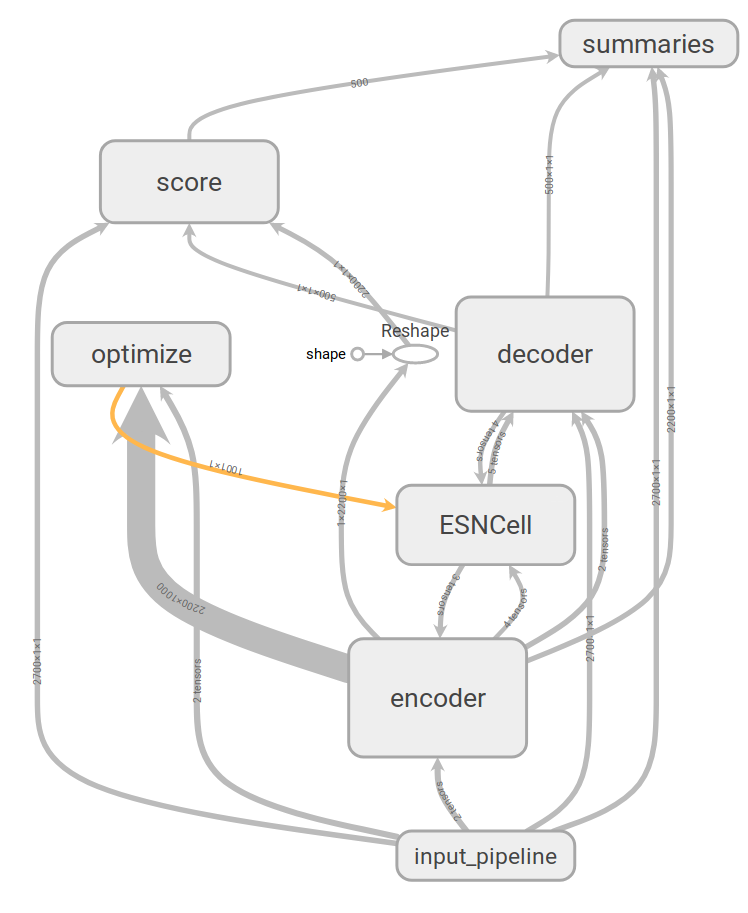
\includegraphics[width=0.8\linewidth]{network_graph.png}
  \caption{Network graph as created by TensorBoard. The nodes represent the
  tensors that hold the actual values of input frames, weight matrices, etc.
  The edges represent the operations, such as multiplications/additions, which
  specify the data flow through the graph. The execution of the specified
  operations is taken care of by Tensorflow. We only need to worry about how
  connect them in a meaningful way.}
  \label{fig:network_graph}
\end{figure}


\begin{enumerate}
  \item \textbf{Read} the input sequence $\mathbf{u}$. Implementation described
    in (Sec.~\ref{sec:input_pipeline}) and represented by the \emph{input
    pipeline} node in the network graph. The input pipelines are defined in
    \ttt{torsk.datasets} and essentially convert Numpy arrays into Tensorflow's
    tensors.

  \item \textbf{Feed} the input sequence $\mathbf{u}$ to the ESN. The ESN cell
    itself, with all its weights is represented by the \emph{ESNCell} node. The
    \emph{encoder} node takes care of looping over the input and feeding it
    frame by frame to the ESN, as well as recording the created internal states
    $\vt{x}$ and ESN outputs $\vt{y}$.

  \item \textbf{Train} the ESN. This is done by the \emph{optimizer} node, which adjusts
    the output weights of the ESN such that the outputs $\vt{y}$ match
    $\vec{u}_{t+1}$ as closely as possible.

  \item \textbf{Predict} the sequence $\mathbf{y}$.  Similarly to step two the
    \emph{decoder} feeds the necessary data to the ESN.  The only difference is
    that now the output of the cell is fed back to its input. This node implements
    the \emph{freely running} ESN.

  \item \textbf{Detect} the eventual anomalies based on $\mathbf{y}$ and
    $\mathbf{d}$.  Described in Sec.~\ref{sec:anomaly_detection_model} and
    represented by the \emph{score} node. The sliding score is implemented both
    in Tensorflow and Numpy in \ttt{torsk.score}.

  \item Evaluate the detected anomalies. This requires human interaction.
\end{enumerate}

The steps 2.-4. are implemented in the \ttt{torsk.models} submodule and
represent most of the logic of the network and the ESN implementations
themselves reside in \ttt{torsk.esn}.  In the following sections we will
revisit the main nodes of the network to describe some specific implementation
details that are worth noting.



\subsection{Input Pipeline}%
\label{sec:input_pipeline}
\begin{listing}
  \inputminted{py}{pseudocode/input_pipeline.py}
  \caption{Simplified input pipeline for sea surface height (SSH) data. The
  lower part of the snippet shows the build phase of a very simple graph and
  how it is executed within a \texttt{tf.Session}.}
  \label{lst:pipeline}
\end{listing}


The goal of the input pipeline is to create an \ttt{inputs} and a \ttt{labels}
sequence that represent the series of inputs $\vt{u}$ and the desired outputs
$\vt{d}$.  The input pipeline takes care of reading slices of the input
sequence to disk and hands them over to the parts of the NN architecture where
it is needed.  There are several ways of doing this in Tensorflow, but the
recommended one is to use the \emph{Dataset API} (\ttt{tf.data.Dataset}).  If
the data is not stored in the TFRecord format a dataset can be created from a
Python generator.  In the case of climate model output they are typically
NetCDF files.  The generator reads in the data, normalizes the values, and
yields time slices of a desired length (Lst.~\ref{lst:pipeline}).  The
generator is now converted into a dataset, which calls the generator as often
as necessary to apply the defined transformations.  The only significant
operation that is applied to the SSH images is resampling them to a desired
size.  To comply with the Tensorflow \emph{Estimator API} the pipeline returns
a dictionary of all features and a single Tensor of labels.  The current input
pipeline is a very simple implementation that was not optimized with regard
to speed, as this was not a bottleneck yet. It might have been sufficient to
just work with \ttt{tf.placeholder} constructs instead.  But because the final
goal was to create an automated detection algorithm that can skim through a lot
of data it seemed feasible to start using the slightly more complicated Dataset
API. In addition, the input functions that are created with the Dataset API can
be used in conjunction with the Estimator API.


\subsection{Echo State Network Cell}%
\label{sec:echo_state_network_cell}

\begin{listing}
  \inputminted{py}{pseudocode/esn_cell.py}
  \caption{Pseudo code for the densely represented ESN cell. The full implementation
  is located at \ttt{torsk.esn.esn\_cell}.}
  \label{lst:esn_cell}
\end{listing}

The central part of the anomaly detection algorithm is the ESN cell, as
governed by the state space equations, which where introduced in
Sec.~\ref{ssub:state_space_model}. It is implemented both in a dense
representation in the \ttt{ESNCell} and a sparse respresentation in the
\ttt{SparseESNCell}.  To create an RNN in Tensoflow's computational graph, it
has to be unrolled along the time axis. For standard RNN tasks the graph
creation is conveniently handled by the \ttt{tf.nn.dynamic\_rnn} function,
which only needs a \ttt{tf.nn.rnn\_cell.RNNCell} object and some inputs to
work.  The ESN cell is implemented as a subclass of the
\ttt{tf.contrib.rnn.LayerRNNCell}, which in turn is a subclass of the RNNCells
to make them act like proper \ttt{tf.Layer} objects.  An RNNCell needs to
implement the \ttt{state\_size} and \ttt{output\_size} properties, as well as a
\ttt{build} and a \ttt{call} method.  The build method initializes all the
weights that are needed in the call method, which defines the operations are
executed at each time step of the RNN.  In most Tensorflow RNN cells the output
weights are defined outside the cell class as they are not part of the
recurrency. The reasons for including them, as well as the state variable that
is returned twice by the call method, will become clear during the section on
the encoder and decoder of the network (Sec.~\ref{sec:encoder_decoder}).
Pseudo code for the ESNCell is given in Lst.~\ref{lst:esn_cell}.

The initialization of the ESN reservoir is done via a custom
\ttt{ESNReservoirIntitializer}.  It inherits from the standard Tensorflow
\ttt{Initializer} class and essentially calls a function that creates a
reservoir matrix in Numpy and converts it to a \ttt{tf.Tensor}.


\subsection{Encoder \& Decoder}%
\label{sec:encoder_decoder}

\begin{listing}[t]
  \inputminted{py}{pseudocode/build_model.py}
  \caption{Functions that create the prediction helper and decoder to feed the
  output of the ESN back to the input.}
  \label{lst:decoder}
\end{listing}

The encoders and decoders of an RNN take over the task of feeding the right
inputs to the network during the training (encoder) and prediction (decoder)
phases. The names encoder and decoder stem from the primary application of RNNs to
natural language processing tasks.  In language processing every word needs to
be encoded into a (typically binary) vector representation before it can be fed
to the network, hence the name. In our case the only thing the encoder does is
to feed the true input $\vt{u}$ to the network and to record the corresponding
output $\vt{y}$ for every frame in the input sequence. This is normally done by
the \ttt{tf.nn.dynamic\_rnn} function.  The decoder is used during the
prediction phase of the network.  It takes care of feeding the current
prediction $\vt{y}$ back to the ESN as the next input $\vec{u}_{t+1}$, which is
not possible with the dynamic RNN encoder.  Instead, the
\ttt{tf.contrib.seq2seq.dynamic\_decode} (line 35 of Lst.~\ref{lst:decoder})
routine can be used. It unrolls the ESN based on a decoder object, which in
turn needs a helper to define the next inputs and the state of the ESN.
Unfortunately, the \ttt{dynamic\_decode} function only returns, apart from
the prediction, the final state of the ESN and none of the intermediate states.
This is a major inconvenience for ESN validation, which is why the custom ESN
cells (Sec.~\ref{sec:echo_state_network_cell}) return the state variable twice.
This way they are treated like outputs, collected at every step, and
returned together with the cell outputs in the end.  Unfortunately, the
practical realization of this idea is a slightly tedious task in Tensorflow
that includes creating a custom \emph{helper}, which, at the time of writing,
are rather sparsely documented.  However, it can be done as shown in
Lst.~\ref{lst:decoder}. The \ttt{prediction\_helper} function defines three
functions that are needed to create a custom helper, which define the behaviour
of the helper during the unroll of the ESN.  Custom helpers quite some
flexibility, including sampling next inputs from either labels (desired
outputs) or predicted outputs, but this is not needed here, so \ttt{sample\_fn}
just returns an arbitrary value.  The \ttt{next\_inputs\_fn} function is called
at each prediction step with the previous cell output as one of its input
arguments.  The important thing is that on line 20 of Lst.~\ref{lst:decoder}
only the current prediction $\vt{y}$ is picked as the next input.
Unfortunately, the extraction of all the intermediate states from the decoder
involves changing the return statement of the ESN cells, which breaks them for
the usage with \ttt{tf.nn.dynamic\_rnn}. To fix this, Tensorflow's decoder
features are used as encodeers by defining another dynamic decoding helper to
return inputs instead of predictions.  The few minor changes that have to be
made to the helper can be found in the repository [\cite{coderepo}].



\subsection{Weight Optimization}%
\label{sec:weight_optimization}

The actual learning of the ESN is carried out by optimizing only the output
weights $\wmatr{out}$ of the cell, which can be achieved via the pseudo-inverse
method or Tikhonov Regularization (Sec.~\ref{sub:esn_training}). The
implementation of either of the two approaches is quite straight forward
and can be found in the two functions \ttt{pseudo\_inverse} and \ttt{tikhonov}
of \ttt{torsk.models.lms}.
Alternatively, the \ttt{torsk.models.grad} submodule implements the network
with Tensorflows gradient optimizers.\\

\subsection{Anomaly Detection}%
\label{sec:anomaly_detection_model}

The anomaly detection, meaning the calculation of the anomaly score, can either
be done online within the network graph, or offline by reading execution
summaries and processing them. The former needs to be implemented in Tensorflow
and is found in \ttt{torsk.score.tfscore}. The latter can be done in Numpy
resides in \ttt{torsk.score.npscore}.  It is a simple function that receives
the prediction errors and a \ttt{large\_window\_size} and a
\ttt{small\_window\_size}, from which the normality score can be calculated
according to Eq.~\ref{eq:normality_score}.

If the anomaly detection is to be done in an online fashion, it needs to be
included into Tensorflow's computational graph.  The anomaly score is based on
a sliding error window, so we need a loop. To prevent a redundant addition of
operations to the graph Tensorflow provides the \ttt{tf.while\_loop} function
to create loops. It needs to be supplied with a conditional function that
defines the stopping criterion and a loop body.  The loop body computes the
anomaly score. Note lines 21-22 where the computed anomaly score is injected
into the \ttt{scores} variable by slicing and concatenation. This needs to be
done this way because the \ttt{tf.assign} operation does not work as expected
in a \ttt{tf.while\_loop}.  The shape of the \ttt{scores} must be reset after
the concatenation in order to convince Tensorflow that the shape is invariant
over the whole loop.

\begin{listing}
  \inputminted{py}{pseudocode/score.py}
  \caption{Tensorflow normality score implementation.}
  \label{lst:score}
\end{listing}


\section{Hyper-Parameter Optimization}%
\label{sec:impl_hyper_parameter_optimization}

The choice of Hyper-parameters of a NN can either be done manually or with a
number of different HP optimization algorithms (is it not a part of a node in
\ref{fig:network_graph}). The most commonly used approach is probably Bayesian
Optimization (as described in Sec.~\ref{sub:bayesian_optimization}).  The
package `scikit-optimize' provides a convenient implementation, whose usage is
sketched in Lst.~\ref{lst:bayes_opt}.  The optimization is launched in line 38
by the \ttt{skopt.gp\_minimize} (Gaussian Process minimize) function. The
essential arguments to this call are the fitness function, the search dimension
specification, and the initial values for each HP.  At each step, the GP
minimizer samples new evaluation parameters from the specified HP dimensions.
They are chosen based on one of three acquisition functions (PI, EI, LCB),
which is indicated by the argument \ttt{"gp\_hedge"}. The algorithm
probabilistically chooses one of the three available acquistion functions.  The
resulting \ttt{sample\_params} are passed to the fitness function, which
optimizes the output weights and creates ten test predictions.  The prediction
error over all predictions is averaged to obtain a metric that reflects the
performance of the currently evaluated HPs. In the case that the predictions
diverge the metric is set to a large finite value.

\begin{listing}
  \inputminted{py}{pseudocode/hparam_opt.py}
  \caption{Bayesian optimization script based on the package [\cite{skopt}].}
  \label{lst:bayes_opt}
\end{listing}
